\documentclass{article}
\usepackage{amsmath}
\usepackage{graphicx}
\usepackage{float}
\usepackage{listings}
\usepackage{caption}
\usepackage{comment}
\usepackage[linesnumbered,vlined]{algorithm2e}
\usepackage{hhline}
\usepackage{geometry}
\usepackage{tabularx}
\usepackage{hyperref}
\usepackage[table]{xcolor}
\usepackage{tcolorbox}
\usepackage{booktabs}
\usepackage{enumitem}
\usepackage[export]{adjustbox}

\title{\textbf{PoolManager}}
\author{Alessandro Aldo Raoul Bonciani}
\date{June 2024}

\begin{document}
 \maketitle

    \vspace{-1em}

    \begin{figure}[h]
        \begin{minipage}{\textwidth}
            \centering
            \includegraphics[width=3cm]{Images/unifi-logo.png}
        \end{minipage}
        \label{fig:uni-logo}
    \end{figure}

\newpage
\tableofcontents
\newpage


\section{Introduzione}\label{sec:introduzione}
Elaborato per il superamento dell'esame di Ingegneria del Software, appartenente al modulo Basi di Dati/Ingegneria del Software del corso di laurea Triennale in Ingegneria Informatica presso l'Università degli Studi di Firenze.
\newline
\newline
Il progetto è stato sviluppato da Alessandro Aldo Raoul Bonciani, matricola 7079209, nel periodo tra maggio - giugno 2024 (a.a. 2023-2024).
\newline
\newline
Il codice sorgente è disponibile su \textit{GitHub} al seguente indirizzo:
\newline
\hyperlink{https://github.com/alebonch/PoolManager}{https://github.com/alebonch/PoolManager}
\subsection{Obiettivo e descrizione del progetto}\label{subsec:obiettivo}
Con questo progetto si sviluppa un programma adibito alla gestione delle prenotazioni di postazioni per la balneazione in un impianto natatorio. 
\newline
Si ha quindi un sistema in cui, utenti e admin, possono inserire prenotazioni andando a richiedere un numero di risorse per la propria postazione.
Inoltre, il sistema di amministrazione, a cui si accede come admin, permette di modificare dati di utenti e la disponibilità delle risorse. Per gestire i dati e salvarli, il programma è stato connesso ad un database.
\subsection{Struttura e pratiche utilizzate}\label{subsec:struttura-e-pratiche-utilizzate}
   Il software è stato sviluppato in Java, mentre per la gestione e il salvataggio dei dati è stato connesso un database PostgreSQL ed è stata utilizzata
            la libreria JDBC (Java DataBase Connectivity). \\

            \noindent Per mantenere una separazione delle responsabilità, la struttura del progetto è stata divisa in tre parti principali: Business Logic, Domain Model e ORM.
            Questi tre packages si occupano in modo distinto della logica di business, della rappresentazione dei dati e dell'accesso ai dati (Figura~\ref{fig:package-dependency-diagram}):
            \begin{itemize}
                \item \textbf{Business Logic}: contiene le classi che implementano la logica di business del sistema.
                \item \textbf{Domain Model}: contiene le classi che rappresentano le entità del sistema.
                \item \textbf{ORM}: contiene le classi che implementano l'Object-Relational Mapping. In questo modo è possibile rendere
                                    i dati persistenti e recuperarli dal database.
            \end{itemize}

            \noindent Per utilizzare il software è stata creata un'interfaccia da riga di comando (CLI) che permette di interagire con il sistema in modo semplice e intuitivo. \\

            \noindent Gli Use Case Diagram e i Class Diagram seguono lo standard UML (Unified Modeling Language) e sono stati realizzati con il software StarUML. \\

            \noindent Le piattaforme e i software utilizzati sono stati:
            \begin{itemize}
                \item \textbf{VisualStudio Code}: IDE per lo sviluppo in Java
                \item \textbf{StarUML}: software per la creazione di diagrammi UML
                \item \textbf{PgAdmin}: software per la gestione di database PostgreSQL
                \item \textbf{GitHub}: piattaforma per la condivisione del codice sorgente
                \item \textbf{Lunacy}: software per la creazione di mock-up
                \item \textbf{Draw.io}: sito che è stato utilizzato per creare il navigation diagram.
                \item \textbf{Overleaf.com}: sito per la creazione di file latex
                % is there anything else?
            \end{itemize}

            \begin{figure}[H]
                \centering
                \fbox{
                    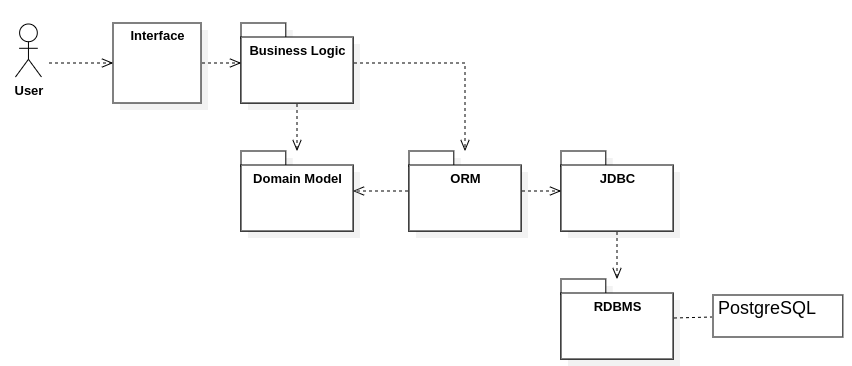
\includegraphics[width=\textwidth]{Images/packages&diagrams/packages.png}
                }
                \caption{Package Dependency Diagram}
                \label{fig:package-dependency-diagram}
            \end{figure}
\section{Progettazione}\label{sec:progettazione}
\subsection{Use case diagram}\label{subsec:use-case-diagram}
Come precedentemente descritto, il sistema permette agli utenti di effettuare prenotazioni di postazioni in determinati turni di una giornata e di gestire il proprio profilo. La seguente immagine mostra il diagramma dei casi di uso del sistema sia per gli utenti che la parte amministrativa. 
\clearpage
\begin{figure}%[H]
                \centering
                \fbox{
                    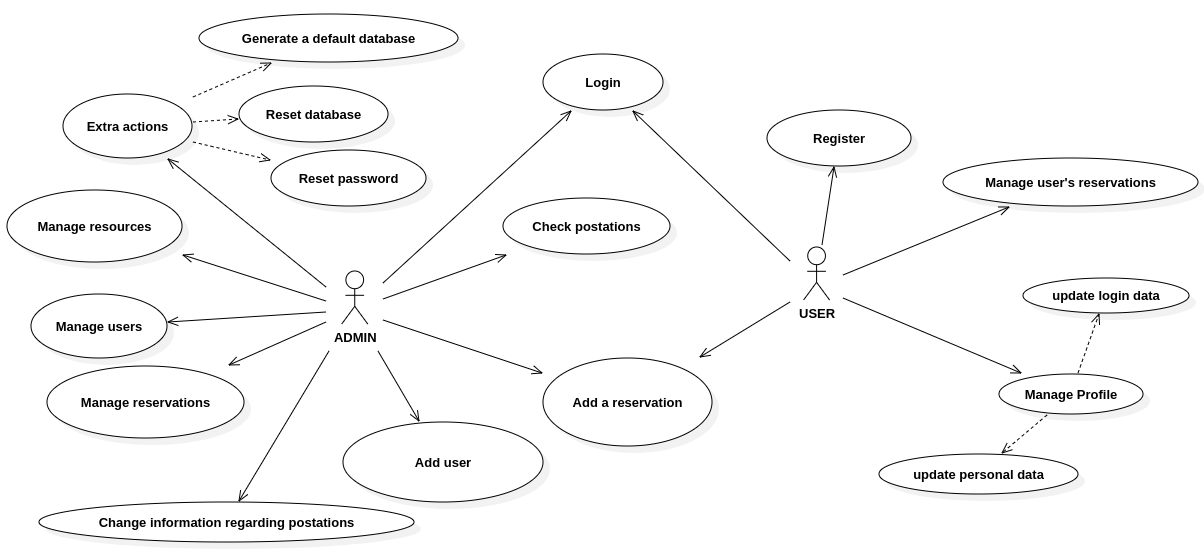
\includegraphics[width=\textwidth]{Images/packages&diagrams/use-case-diagram.png}
                }
                \caption{Use Case Diagram}
                \label{fig:use-case-diagram}
            \end{figure}
\subsection{Use case template}\label{subsec:use-case-template}
Di seguito sono riportati i template di alcuni dei casi d'uso implementati, in ognuno possiamo trovare: una breve descrizione,
il livello del caso d'uso, gli attori coinvolti, le pre-condizioni, le post-condizioni, il flusso base e i flussi alternativi. \\
\clearpage
\vspace{0.5cm}

            \renewcommand{\arraystretch}{1.5}

            % Use Case Template 1
            %\resizebox{0.8\textwidth}{!}{
            \begin{table}[h]
                \centering
                %\resizebox{0.9\textwidth}{!}{
                \small
                \begin{tabularx}{\textwidth}{|lX|}
                    %\bottomrule
                    %\rowcolor{white} \textbf{Use Case \#1} & \textbf{Accesso al sistema (Sign in)} \\
                    \multicolumn{1}{l}{\rowcolor{grey!20} \textbf{Use Case \#1}} & \multicolumn{1}{l}{\textbf{Accesso al sistema (Log-in)}} \\
                    \bottomrule
                    \rowcolor{white} \textbf{Brief Description} & L'utente accede al sistema tramite le proprie credenziali (\hyperref[fig:mockup-login]{\small{Mockup Login}}, \hyperref[fig:logintest]{\small{LoginControllerTest}}) \\
                    %\midrule
                    \rowcolor{blue!10} \textbf{Level} & Function \\
                    %\midrule
                    \rowcolor{white} \textbf{Actors} & Utente, Admin \\
                    %\midrule
                    \rowcolor{blue!10} \textbf{Pre-conditions} & L'utente deve essere nella pagina iniziale di accesso.  \\
                    %\midrule
                    \rowcolor{white} \textbf{Basic Flow} & \begin{description}[nosep,before=\leavevmode\vspace*{-1\baselineskip},after=\leavevmode\vspace*{-1\baselineskip}]
                                                               \item [1.] L'utente inserisce le proprie credenziali (username e password)
                                                               \item [2.] L'utente preme il pulsante di accesso
                                                               \item [3.] Il sistema verifica le credenziali
                                                               \item [4.] Il sistema autentica l'utente
                                                           \end{description} \\
                    %\midrule
                    \rowcolor{blue!10} \textbf{Alternative Flows} & \begin{description}[nosep,before=\leavevmode\vspace*{-1\baselineskip},after=\leavevmode\vspace*{-1\baselineskip}]
                                                                        \item [3a.] Se le credenziali fornite non sono corrette, il sistema mostra un messaggio di errore all'utente
                                                                        \item [4a.] Se a fare l'accesso è l'admin, il sistema lo reindirizza alla Admin Page (\small{TST \#03})
                                                                    \end{description} \\
                    %\midrule
                    \rowcolor{white} \textbf{Post-conditions} & L'utente è autenticato nel sistema e ha accesso alle funzionalità riservate \\
                    %\bottomrule
                    \toprule
                \end{tabularx}
                %}
                %\captionsetup{font=small,labelfont=bf}
                \caption{Use Case Template 1 (Sign in)}
                \label{tab:use-case-template-1}
            \end{table}
            %}
            \clearpage
             % Use Case Template 2
            \begin{table}%[h]
                \centering
                %\resizebox{0.9\textwidth}{!}{
                \small
                \begin{tabularx}{\textwidth}{|lX|}
                    %\bottomrule
                    %\rowcolor{white} \textbf{Use Case \#2} & \textbf{Registrazione nel sistema (Sign up)} \\
                    \multicolumn{1}{l}{\rowcolor{grey!20} \textbf{Use Case \#2}} & \multicolumn{1}{l}{\textbf{Registrazione nel sistema (Register)}} \\
                    \bottomrule
                    \rowcolor{white} \textbf{Brief Description} &  L'utente si registra nel sistema creando un nuovo account (\hyperref[fig:registertest]{\small{LoginControllerTest}})\\
                    %\midrule
                    \rowcolor{blue!10} \textbf{Level} & User Goal \\
                    %\midrule
                    \rowcolor{white} \textbf{Actors} & Utente \\
                    %\midrule
                    \rowcolor{blue!10} \textbf{Pre-conditions} & L'utente deve essere nella pagina iniziale di registrazione \\
                    %\midrule
                    \rowcolor{white} \textbf{Basic Flow} & \begin{description}[nosep,before=\leavevmode\vspace*{-1\baselineskip},after=\leavevmode\vspace*{-1\baselineskip}]
                                                               \item [1.] L'utente fornisce i dettagli richiesti per la registrazione
                                                               \item [2.] L'utente conferma la registrazione
                                                               \item [3.] Il sistema verifica i dati forniti
                                                               \item [4.] Il sistema crea un nuovo account per l'utente
                                                           \end{description} \\
                    %\midrule
                    \rowcolor{blue!10} \textbf{Alternative Flows} & \begin{description}[nosep,before=\leavevmode\vspace*{-1\baselineskip},after=\leavevmode\vspace*{-1\baselineskip}]
                                                                        \item [3a.] Se l'utente fornisce dati non validi o se l'email o lo username sono già utilizzati da un altro account, il sistema mostra un messaggio di errore
                                                                    \end{description} \\
                    %\midrule
                    \rowcolor{white} \textbf{Post-conditions} & L'utente è registrato nel sistema e può accedere utilizzando le credenziali create durante la registrazione \\
                    %\bottomrule
                    \toprule
                \end{tabularx}
                %}
                %\captionsetup{font=small,labelfont=bf}
                \caption{Use Case Template 2 (Sign up)}
                \label{tab:use-case-template-2}
            \end{table}
     % Use Case Template 3
            \begin{table}%[h]
                \centering
                %\resizebox{0.9\textwidth}{!}{
                \small
                \begin{tabularx}{\textwidth}{|lX|}
                    %\bottomrule
                    %\rowcolor{white} \textbf{Use Case \#2} & \textbf{Registrazione nel sistema (Sign up)} \\
                    \multicolumn{1}{l}{\rowcolor{grey!20} \textbf{Use Case \#3}} & \multicolumn{1}{l}{\textbf{Creazione di una prenotazione}} \\
                    \bottomrule
                    \rowcolor{white} \textbf{Brief Description} &  L'utente prenota una postazione richiedendo un certo numero di risorse. (\hyperref[fig:mockup-reserve]{\small{Mockup Reserve}}, \hyperref[fig:Admincontrollertestsnippets]{\small{AdminControllerTest}})\\
                    %\midrule
                    \rowcolor{blue!10} \textbf{Level} & User Goal \\
                    %\midrule
                    \rowcolor{white} \textbf{Actors} & Utente, Admin \\
                    %\midrule
                    \rowcolor{blue!10} \textbf{Pre-conditions} & L'utente deve essere nella pagina di gestione delle prenotazione \\
                    %\midrule
                    \rowcolor{white} \textbf{Basic Flow} & \begin{description}[nosep,before=\leavevmode\vspace*{-1\baselineskip},after=\leavevmode\vspace*{-1\baselineskip}]
                                                               \item [1.] L'utente fornisce i dettagli richiesti per la prenotazione
                                                               \item [2.] Il sistema verifica che la richiesta sia accettabile
                                                               \item [3.] Il sistema calcola il costo della prenotazione
                                                               \item [4.] Il sistema crea una nuova prenotazione, una postazione e la inserisce nel database
                                                           \end{description} \\
                    %\midrule
                    \rowcolor{blue!10} \textbf{Alternative Flows} & \begin{description}[nosep,before=\leavevmode\vspace*{-1\baselineskip},after=\leavevmode\vspace*{-1\baselineskip}]
                                                                        \item [3a.] Se l'utente richiede troppe risorse, il sistema genera dei messaggi di errore 
                                                                    \end{description} \\
                    %\midrule
                    \rowcolor{white} \textbf{Post-conditions} & La prenotazione viene inserita nel sistema e il numero di risorse disponibili in quel time record diminuirà in base alla richiesta \\
                    %\bottomrule
                    \toprule
                \end{tabularx}
                %}
                %\captionsetup{font=small,labelfont=bf}
                \caption{Use Case Template 3 (Reserve)}
                \label{tab:use-case-template-3}
            \end{table}
 %Use Case Template 4
            \begin{table}%[h]
                \centering
                %\resizebox{0.9\textwidth}{!}{
                \small
                \begin{tabularx}{\textwidth}{|lX|}
                    %\bottomrule
                    %\rowcolor{white} \textbf{Use Case \#8} & \textbf{Ripristino del database} \\
                    \multicolumn{1}{l}{\rowcolor{grey!20} \textbf{Use Case \#4}} & \multicolumn{1}{l}{\textbf{Ripristino del database}} \\
                    \bottomrule
                    \rowcolor{white} \textbf{Brief Description} & L'Admin esegue l'operazione di ripristino del database  (\hyperref[fig:Admincontrollertestsnippets]{\small{AdminControllerTest}})\\
                    %\midrule
                    \rowcolor{blue!10} \textbf{Level} & Function \\
                    %\midrule
                    \rowcolor{white} \textbf{Actors} & Admin \\
                    %\midrule
                    \rowcolor{blue!10} \textbf{Pre-conditions} &  L'Admin ha effettuato l'accesso al sistema \\
                    %\midrule
                    \rowcolor{white} \textbf{Basic Flow} & \begin{description}[nosep,before=\leavevmode\vspace*{-1\baselineskip},after=\leavevmode\vspace*{-1\baselineskip}]
                                                               \item [1.] L'amministratore seleziona l'opzione per il ripristino del database
                                                               \item [2.] L'amministratore conferma l'avvio del processo di ripristino
                                                               \item [3.] Il sistema esegue il ripristino del database
                                                               \item [4.] Il sistema conferma all'amministratore che il ripristino è stato completato con successo
                                                           \end{description} \\
                    %\midrule
                    \rowcolor{blue!10} \textbf{Alternative Flows} & \begin{description}[nosep,before=\leavevmode\vspace*{-1\baselineskip},after=\leavevmode\vspace*{-1\baselineskip}]
                                                                        \item [3a.] Se il processo di ripristino del database fallisce per qualsiasi motivo, il sistema mostra un messaggio di errore all'amministratore
                                                                    \end{description} \\
                    %\midrule
                    \rowcolor{white} \textbf{Post-conditions} & Il database è stato ripristinato con successo \\
                    %\bottomrule
                    \toprule
                \end{tabularx}
                
                %\captionsetup{font=small,labelfont=bf}
                \caption{Use Case Template 4 (Reset database)}
                \label{tab:use-case-template-4}
            \end{table}
            \clearpage

            
\subsection{Mockups}\label{subsec:mockups}
Di seguito si inseriscono alcuni possibili Mock-ups relativi alle interfacce grafiche del sistema.


\clearpage
\setlength{\fboxsep}{0pt}
            \begin{figure}%[H]
                \centering
                \resizebox{0.98\textwidth}{!}{
                \setlength{\fboxsep}{0pt} % Adjust to your preference
                \tcbox[colframe=darkgrey!30,colback=darkgray!20,boxsep=0mm,arc=0mm]{ % Change 'darkgray' to your preferred color, adjust 'arc' for roundness
                    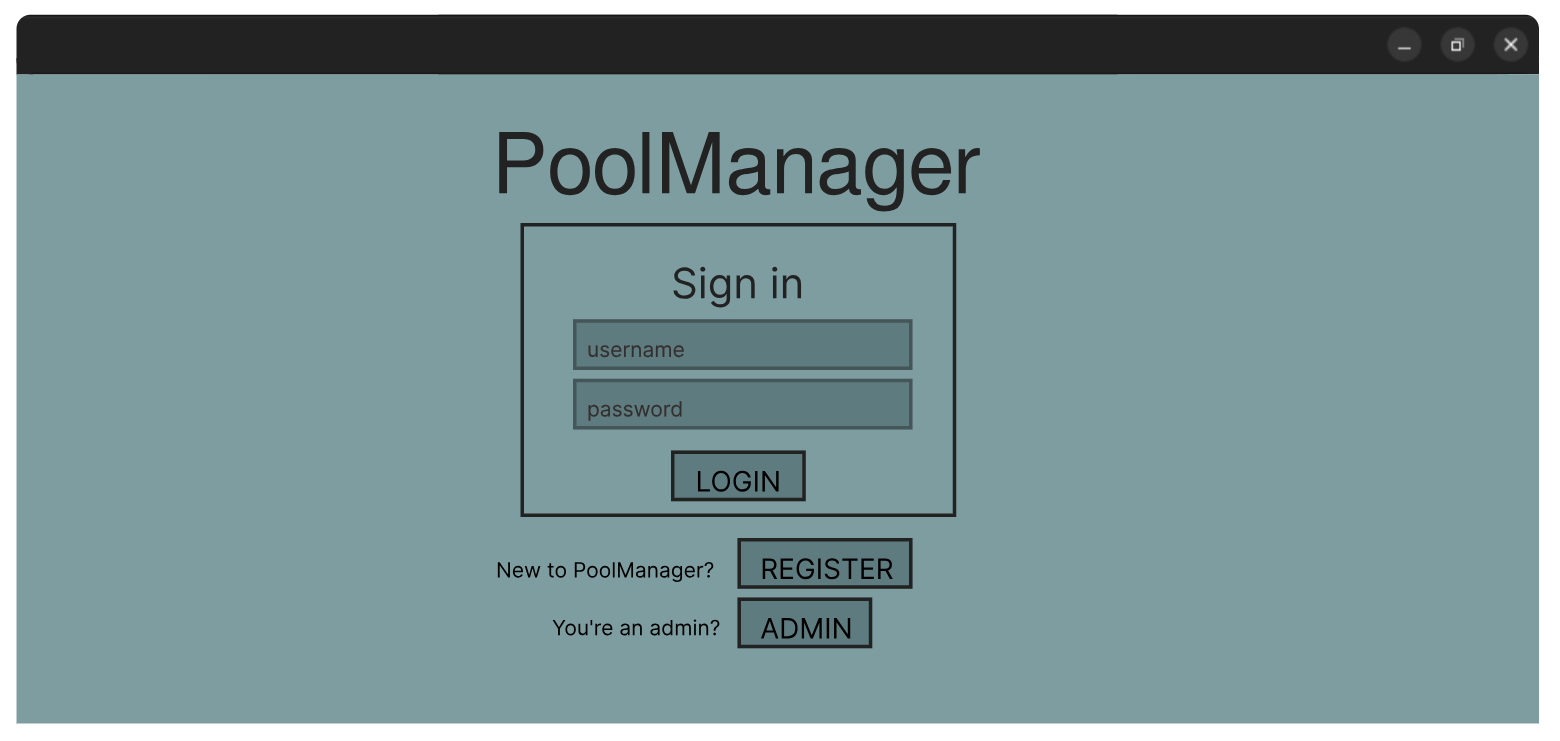
\includegraphics[width=\textwidth]{Images/Mockups/Mockup-login.png} % Adjust the width to your preference
                }
                }
                \caption{Prototipo della pagina di login / registrazione}
                \label{fig:mockup-login}
            \end{figure}
\setlength{\fboxsep}{0pt}
            \begin{figure}%[H]
                \centering
                \resizebox{0.98\textwidth}{!}{
                \setlength{\fboxsep}{0pt} % Adjust to your preference
                \tcbox[colframe=darkgrey!30,colback=darkgray!20,boxsep=0mm,arc=0mm]{ % Change 'darkgray' to your preferred color, adjust 'arc' for roundness
                    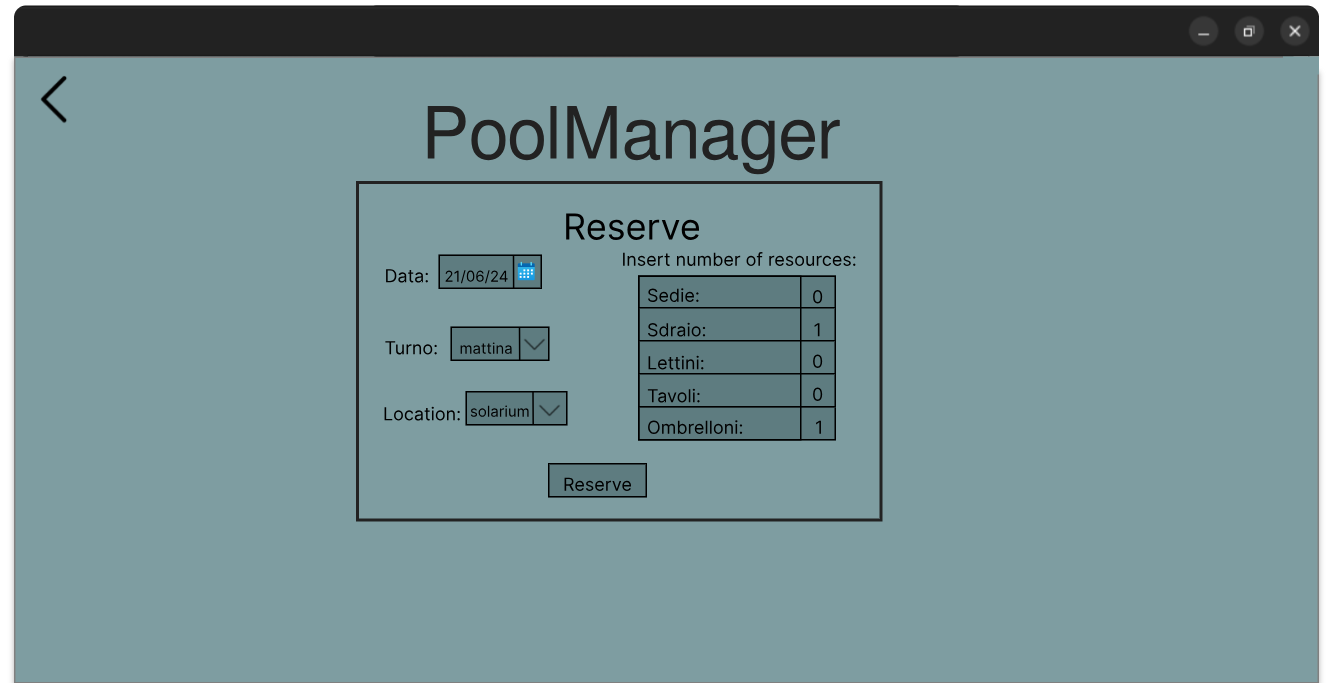
\includegraphics[width=\textwidth]{Images/Mockups/Mockup-reserve.png} % Adjust the width to your preference
                }
                }
                \caption{Prototipo della pagina di prenotazione}
                \label{fig:mockup-reserve}
            \end{figure}
            \setlength{\fboxsep}{0pt}
            \begin{figure}%[H]
                \centering
                \resizebox{0.98\textwidth}{!}{
                \setlength{\fboxsep}{0pt} % Adjust to your preference
                \tcbox[colframe=darkgrey!30,colback=darkgray!20,boxsep=0mm,arc=0mm]{ % Change 'darkgray' to your preferred color, adjust 'arc' for roundness
                    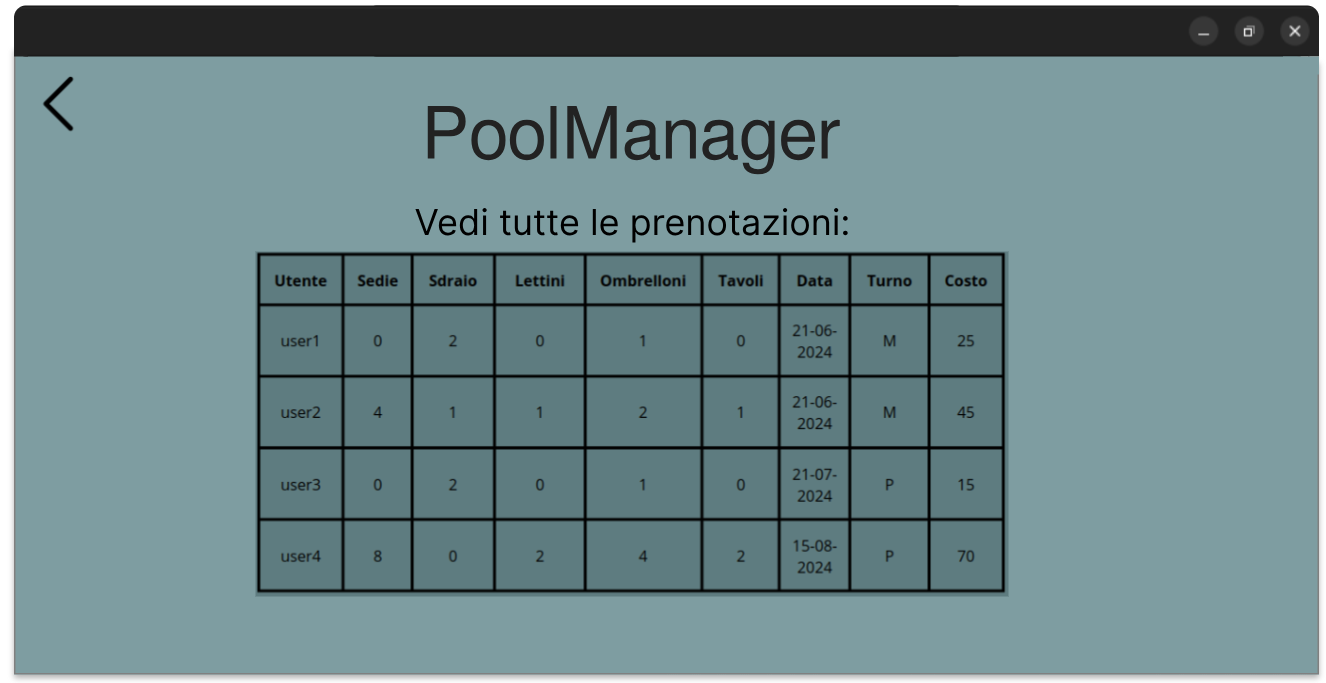
\includegraphics[width=\textwidth]{Images/Mockups/Mockup-view.png} % Adjust the width to your preference
                }
                }
                \caption{Prototipo della pagina di visione delle prenotazioni}
                \label{fig:mockup-view}
            \end{figure}
            \clearpage
\subsection{Class diagram}\label{subsec:class-diagram}
Vista la divisione strutturale in 3 packages, sono stati realizzati 3 diagrammi delle classi distinti, uno per ogni package:
            \begin{itemize}
                \item \textbf{Business Logic} (Figura~\ref{fig:business-logic-class-diagram}): contiene le classi che implementano la logica di business del sistema, ovvero i seguenti controller:
                    quello che gestisce l'accesso e la registrazione dei nuovi utenti (\texttt{LoginController}),
                    quello che permette agli utenti aggiornare i propri dati e controllare le proprie prenotazioni (\texttt{UserController}),
                    quello che permette di creare e modificare le proprie prenotazioni (\texttt{ReserveController}),
                    quello che permette di gestire le risorse disponibili e controllarne la disponibilità (\texttt{ResourcesController}),
                    quello che gestisce le azioni dell'admin  (\texttt{AdminController})
                \item \textbf{Domain Model} (Figura~\ref{fig:domain-model-class-diagram}): contiene le classi che rappresentano le entità del sistema, ovvero:
                    \texttt{User}, \texttt{Object}, \texttt{Chair}, \texttt{Deckchair}, \texttt{Sunbed}, \texttt{Table}, \texttt{Umbrella}, \texttt{Reservation}, \texttt{Postation}, \texttt{Location} e \texttt{TimeRecord}, .
                \item \textbf{ORM} (Figura~\ref{fig:orm-class-diagram}): contiene le classi che implementano l'Object-Relational Mapping, quindi contiene una classe per ogni entità del sistema:
                    \texttt{UserDAO}, \texttt{ObjectDAO}, \texttt{PostationDAO}, \texttt{ReservationDAO}, \texttt{TimeRecordDAO} e \texttt{LocationDAO}.
                    In più contiene anche la classe \texttt{AdminDAO} che si occupa della gestione dei dati dell'admin
                    e la classe \texttt{ConnectionManager} che si occupa di gestire la connessione al database.
            \end{itemize}

            \begin{figure}[H]
                \centering
                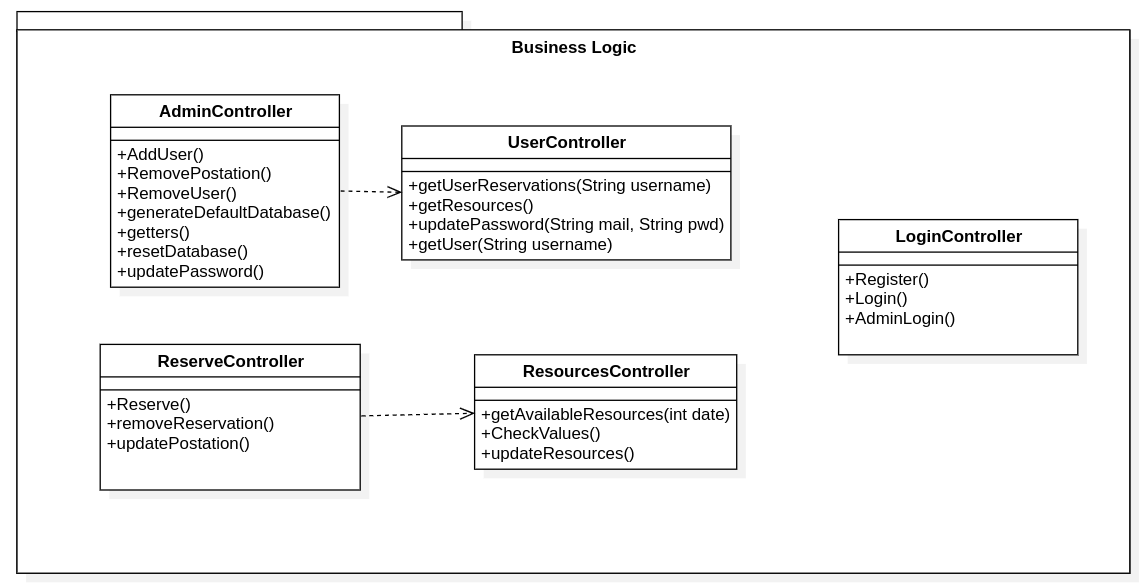
\includegraphics[width=\textwidth]{Images/packages&diagrams/Business Logic.png}
                \caption{Class Diagram - Business Logic}
                \label{fig:business-logic-class-diagram}
            \end{figure}

            \clearpage

            \begin{figure}[H]
                \centering
                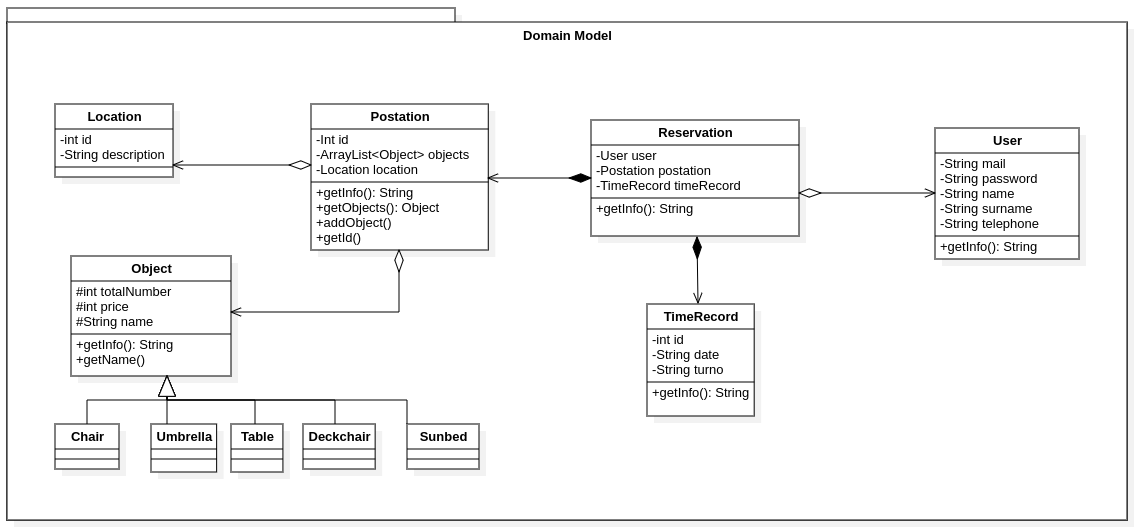
\includegraphics[width=\textwidth]{Images/packages&diagrams/Domain Model.png}
                \caption{Class Diagram - Domain Model}
                \label{fig:domain-model-class-diagram}
            \end{figure}

            \begin{figure}[H]
                \centering
                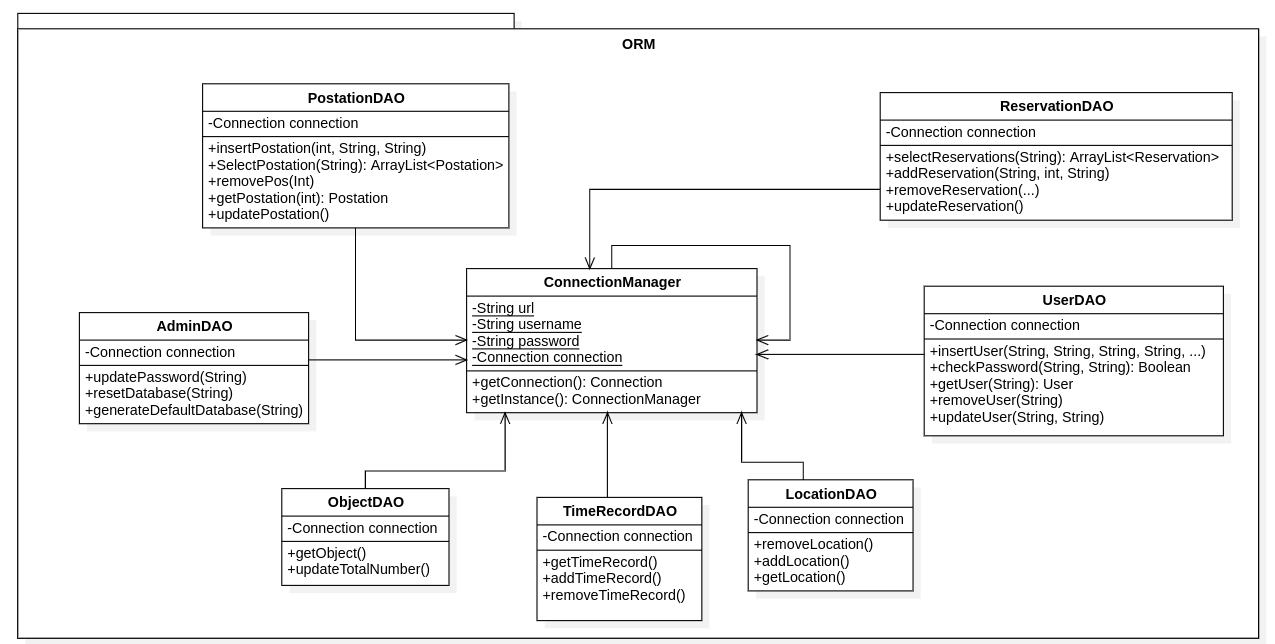
\includegraphics[width=\textwidth]{Images/packages&diagrams/ORM.png}
                \caption{Class Diagram - ORM}
                \label{fig:orm-class-diagram}
            \end{figure}
\clearpage
\subsection{ER Diagram e modello relazionale}\label{subsec:ERdiagram}
Per quanto riguarda la progettazione del database (\ref{fig:er-diagram-1}), si hanno queste entità:
\begin{itemize}
     \item \texttt{User}: rappresenta l'entità \texttt{User}.
            \item \texttt{Postation}: rappresenta l'entità \texttt{Postation}. L'ArrayList di oggetti che è presente all'interno della classe (\ref{fig:domain-model-class-diagram}) è stato inserito inserendo come colonne ogni singolo possibile valore presente tra gli oggetti.
            \item \texttt{Reservation}: rappresenta l'entità \texttt{Reservation} e risolve la relazione tra \texttt{User}, \texttt{TimeRecord} e \texttt{Postation}.
            \item \texttt{TimeRecord}: rappresenta l'entità \texttt{TimeRecord}.
            \item \texttt{Location}: rappresenta l'entità \texttt{Location}
            \item \texttt{Object}: rappresenta l'entità \texttt{Object}. A discapito di valori nulli, sono stati inseriti come colonne tutti gli attributi possibili che ogni risorsa può avere.
\end{itemize}

\begin{figure}[H]
                \centering
                \fbox{
                    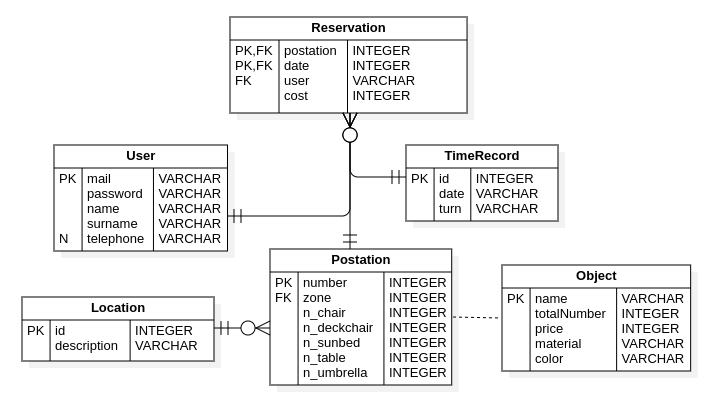
\includegraphics[width=\textwidth]{Images/packages&diagrams/ER diagram.png}
                }
                \caption{ER Diagram RAW view}
                \label{fig:er-diagram-1}
            \end{figure}
            \begin{figure}[H]
                \centering
                \fbox{
                    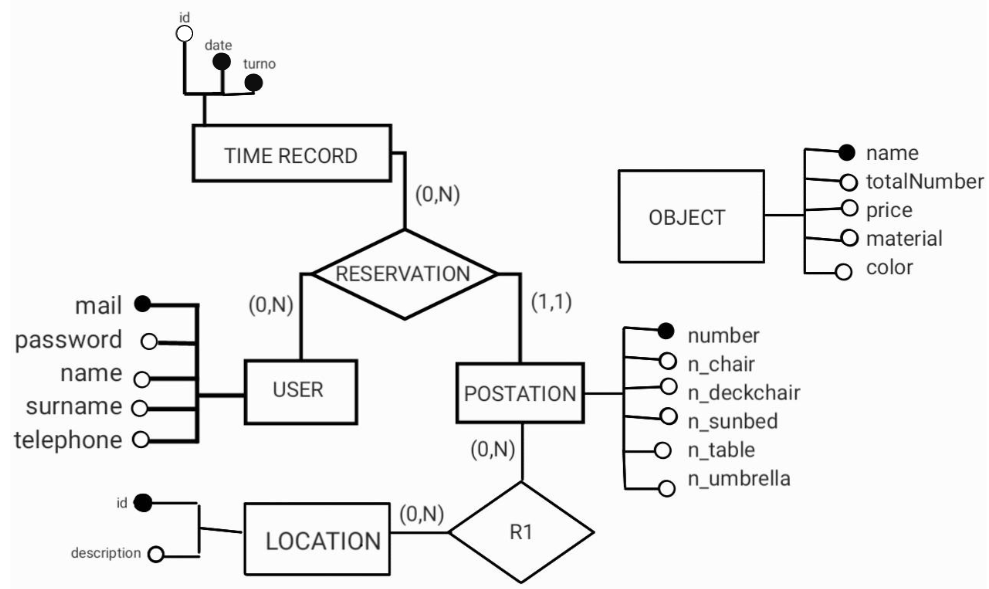
\includegraphics[width=\textwidth]{Images/packages&diagrams/er-diagramRAW.png}
                }
                \caption{ER Diagram}
                \label{fig:er-diagram-2}
            \end{figure}
            \clearpage
\subsection{Navigation Diagram}\label{subsec:navigation-diagram}
Il seguente diagramma (Figura~\ref{fig:navigation-diagram}) rappresenta quelle che sono le pagine principali del sistema e le possibili azioni che l'utente può compiere.
            Sono anche rappresentati i modi con cui si può navigare tra le varie pagine. \\
            Alcune delle pagine sono:
            \begin{itemize}
                \item la pagina iniziale \texttt{PoolManager}: dove l'utente può registrarsi o effettuare il login.
                \item \texttt{User/Admin Reservation Actions}: in cui si può visualizzare prenotazioni, aggiungerne, rimuoverne o modificarne.
                \item \texttt{Event Editor}: la quale permette di creare un nuovo evento o di modificarne uno esistente.
                \item \texttt{User Profile Actions}: dove è possibile modificare i dati di accesso, cambiare dati personali o controllare i dati attuali. 
                \item \texttt{Extra}: dalla quale l'admin può cambiare password o fare il reset del database.
            \end{itemize}
\begin{figure}%[H]
                \centering
                \fbox{
                    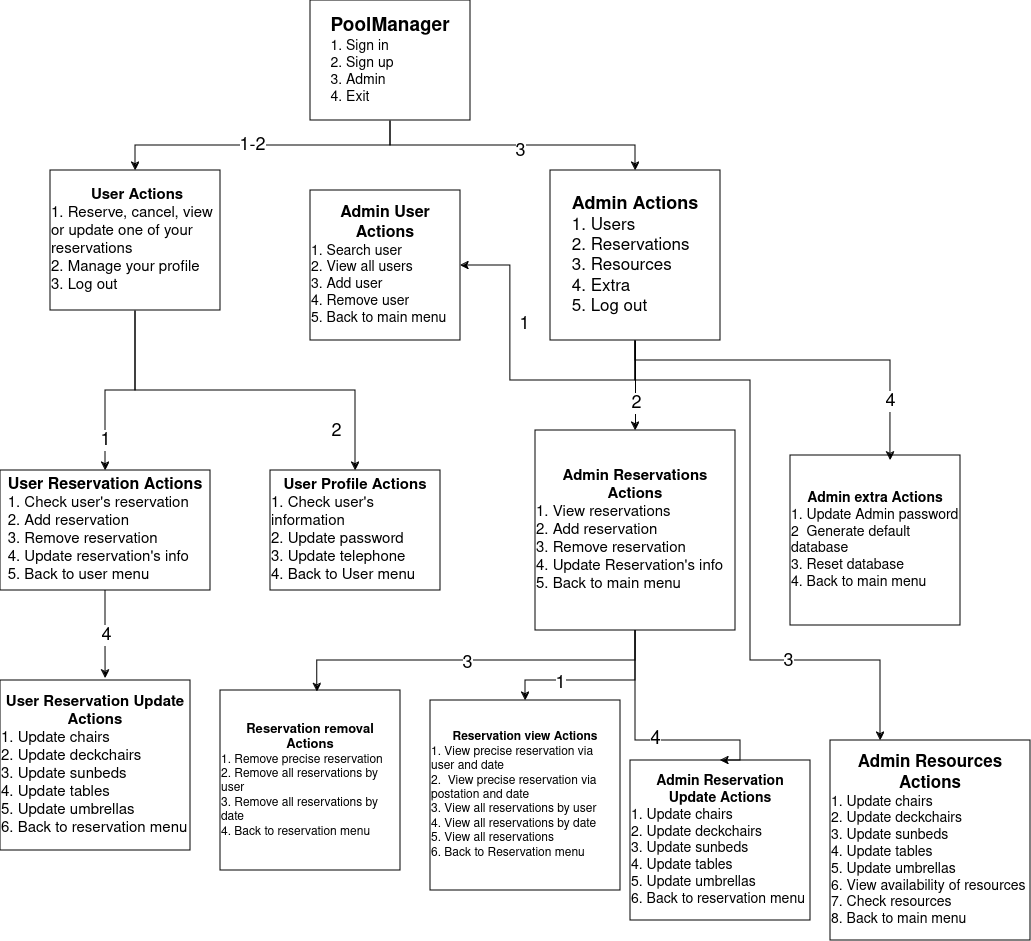
\includegraphics[width=\textwidth]{Images/packages&diagrams/Navigation Diagram.png}
                }
                \caption{Navigation Diagram}
                \label{fig:navigation-diagram}
            \end{figure}
            \clearpage
\section{Implementazione}\label{sec:implementazione}
L'implementazione dei 3 packages \hyperref[subsec:domainmodel]{Domain Model}, \hyperref[subsec:BusinessLogic]{Business Logic} e
\hyperref[subsec:ORM]{ORM} e quella dell'\hyperref[subsec:interfaccia-cli]{interfaccia} sono contenute in \texttt{src/main/java},
mentre i file relativi al \hyperref[subsec:Database]{database} sono contenuti in \texttt{src/main/sql}.
\subsection{Domain Model}\label{subsec:domainmodel}
Come già accennato nella sezione \hyperref[subsec:class-diagram]{2.4}, nel package \texttt{java.DomainModel} (il percorso è:
\texttt{src/java/DomainModel}) sono state implementate le classi che rappresentano le en-
tità del sistema.
\subsubsection{Object}\label{subsubsec:object}
Classe astratta che rappresenta le risorse, ovvero ogni singolo oggetto possibilmente prenotabile da un utente. I suoi attributi sono: \textit{totalNumber}, \textit{price} e \textit{name}.
\subsubsection{Chair}\label{subsubsec:chair}
Specifico oggetto derivato dalla classe \hyperref[subsubsec:object]{Object}. I suoi attributi sono: \textit{color},  \textit{totalNumber}, \textit{price} e \textit{name}.
\subsubsection{Deckchair}\label{subsubsec:deckchair}
Specifico oggetto derivato dalla classe \hyperref[subsubsec:object]{Object}. I suoi attributi sono: \textit{color}, \textit{material},  \textit{totalNumber}, \textit{price} e \textit{name}.
\subsubsection{Sunbed}\label{subsubsec:sunbed}
Specifico oggetto derivato dalla classe \hyperref[subsubsec:object]{Object}. I suoi attributi sono: \textit{material},  \textit{totalNumber}, \textit{price} e \textit{name}.
\subsubsection{Table}\label{subsubsec:table}
Specifico oggetto derivato dalla classe \hyperref[subsubsec:object]{Object}. I suoi attributi sono: \textit{color}, \textit{material},  \textit{totalNumber}, \textit{price} e \textit{name}.
\subsubsection{Umbrella}\label{subsubsec:umbrella}
Specifico oggetto derivato dalla classe \hyperref[subsubsec:object]{Object}. I suoi attributi sono: \textit{color},  \textit{totalNumber}, \textit{price} e \textit{name}.
\subsubsection{TimeRecord}\label{subsubsec:timerecord}
Classe che rappresenta il momento per cui viene fissata la prenotazione. I suoi attributi sono: \textit{id}, \textit{date}, \textit{turn}. Dove \textit{turn} è una stringa il cui valore può essere "mattina" o "pomeriggio".
\subsubsection{Postation}\label{subsubsec:postation}
Classe che rappresenta la postazione richiesta dall'utente nel momento della prenotazione. I suoi attributi sono: \textit{id}, \textit{objects} (un \textit{ArrayList} di \hyperref[subsubsec:object]{oggetti}) e una \hyperref[subsubsec:Location]{\textit{location}}.
\subsubsection{User}\label{subsubsec:user}
Un utente già registrato all'interno del sistema. I campi della classe sono: \textit{mail}, \textit{name}, \textit{surname}, \textit{pwd} e \textit{telephone}.
\subsubsection{Location}\label{subsubsec:Location}
Classe che rappresenta le possibili scelte tra le zone della piscina. I suoi attributi sono: \textit{id}, \textit{description}.
\subsubsection{Reservation}\label{subsubsec:reservation}
Classe che rappresenta la prenotazione. E' formata da: una \hyperref[subsubsec:postation]{\textit{postazione}}, uno \hyperref[subsubsec:user]{\textit{user}}e un \hyperref[subsubsec:timerecord]{\textit{timerecord}}.
\subsection{ORM}\label{subsec:ORM}
Come già accennato nella sezione \hyperref[subsec:class-diagram]{2.4}, nel package \texttt{java.ORM} (il percorso è: \\ \texttt{src/java/ORM})
            sono state implementate le classi che si occupano dell'\textit{Object-Relational Mapping}, ovvero delle  operazioni di lettura e scrittura dei dati nel database.
            Ogni singola classe fuorché \hyperref[subsubsec:connectionmanager]{\textbf{ConnectionManager}} permette alle classi del package \texttt{java.BusinessLogic} di accedere ai dati salvati nel database e possiede come attributo un'istanza di \hyperref[subsubsec:connectionmanager]{\textbf{ConnectionManager}}.
            
\subsubsection{UserDAO}\label{subsubsec:userDAO}
Classe che si occupa della generazione di nuovi utenti attraverso il metodo \textit{insertUser()}, di rimuoverne con \textit{removeUser()}, di aggiornare le informazioni dell'utente e di selezionare utenti. Questa classe si occupa anche del controllo necessario al Login attraverso il metodo \textit{checkPassword()}.
\subsubsection{AdminDAO}\label{subsubsec:adminDAO}
Classe che si occupa delle \hyperref[subsec:navigation-diagram]{Extra actions}, ovvero: reset del database, generazione di un database di default e il cambio di password dell'admin.
\begin{figure}[H]
                \centering
                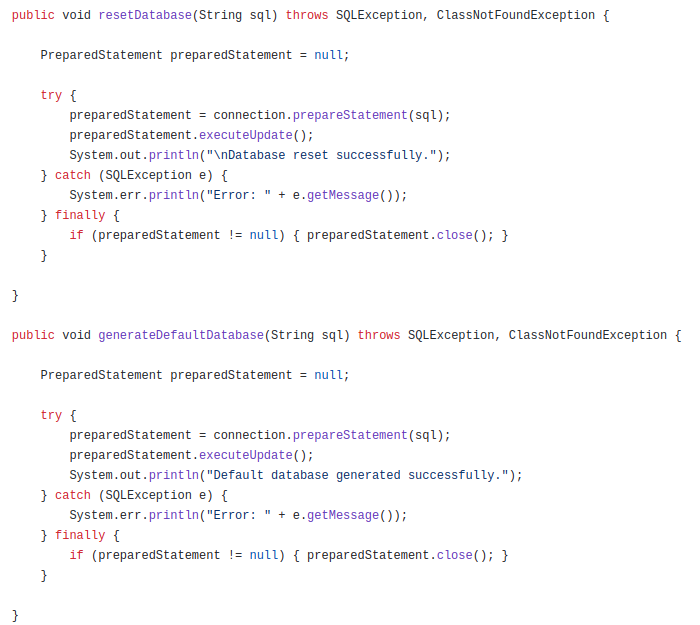
\includegraphics[width=0.9\textwidth]{Images/Snippets/AdminDAO.png}
                \captionsetup{labelformat=empty,labelsep=none}
                \caption{Snippet: implementazione delle Extra actions}
                \label{fig:snippetadmindao}
            \end{figure}
\subsubsection{ObjectDAO}\label{subsubsec:objectDAO}
Classe che si occupa della gestione dei dati che riguardano le risorse.
\subsubsection{TimeRecordDAO}\label{subsubsec:timerecordDAO}
Classe che si occupa della gestione dei singoli \hyperref[subsubsec:timerecord]{\textbf{TimeRecord}}, necessaria per calcolare dinamicamente il numero di risorse utilizzate in un dato \textbf{TimeRecord}.
\subsubsection{LocationDAO}\label{subsubsec:locationDAO}
Classe che si occupa dell'inserimento e rimozione delle \hyperref[subsubsec:Location]{\textit{\textbf{Location}}}.
\subsubsection{PostationDAO}\label{subsubsec:postationDAO}
Classe che si occupa della gestione delle postazioni, oltre ai metodi per aggiungere, rimuovere, aggiornare e selezionare, è presente un ulteriore metodo \textit{getUsedResources()} necessario al calcolo dinamico delle risorse disponibili.
\subsubsection{ReservationDAO}\label{subsubsec:reservationDAO}
Classe che si occupa della gestione delle prenotazioni, in particolare si è voluto aggiungere diversi metodi di rimozione e selezione di modo da poter andare più o meno nello specifico, in base all'esigenza. E' ovviamente presente anche un metodo per aggiungere una \hyperref[subsubsec:reservation]{{\textbf{Reservation}}, senza però alcun controllo sulle risorse, cosa che viene fatta dai controller.
\subsubsection{ConnectionManager}\label{subsubsec:connectionmanager}
La classe si occupa di gestire la connessione al database per le altre classi DAO tramite il metodo \texttt{getConnection()}.
Contiene inoltre i dati di accesso al database, ovvero URL, username e password, che vengono utilizzati per stabilire la connessione.
Per garantire che ci sia una sola istanza della classe in tutto il sistema e quindi per evitare conflitti tra connessioni, la classe è implementata come un \textit{singleton}.


\subsection{Business Logic}\label{subsec:BusinessLogic}
Come già accennato nella sezione \hyperref[subsec:class-diagram]{2.4}, nel package \texttt{java.BusinessLogic}
(il percorso è:
\newline\texttt{src/java/BusinessLogic}) sono state implementate le classi che gestiscono la logica di business del sistema.


\subsubsection{AdminController}\label{subsubsec:admincontroller}
Controller che gestisce le diverse operazioni che possono essere eseguite dall'Actor \textit{Admin}. Si hanno quindi diversi strumenti di selezione per poter controllare tutte le prenotazioni e le postazioni. Inoltre sono qua presenti le \hyperref[fig:admincontrollerSnippets]{Extra Actions}. Per alcune operazioni, chiama \hyperref[subsubsec:usercontroller]{\textbf{UserController}} e ne utilizza i metodi.
\begin{figure}[H]
                \centering
                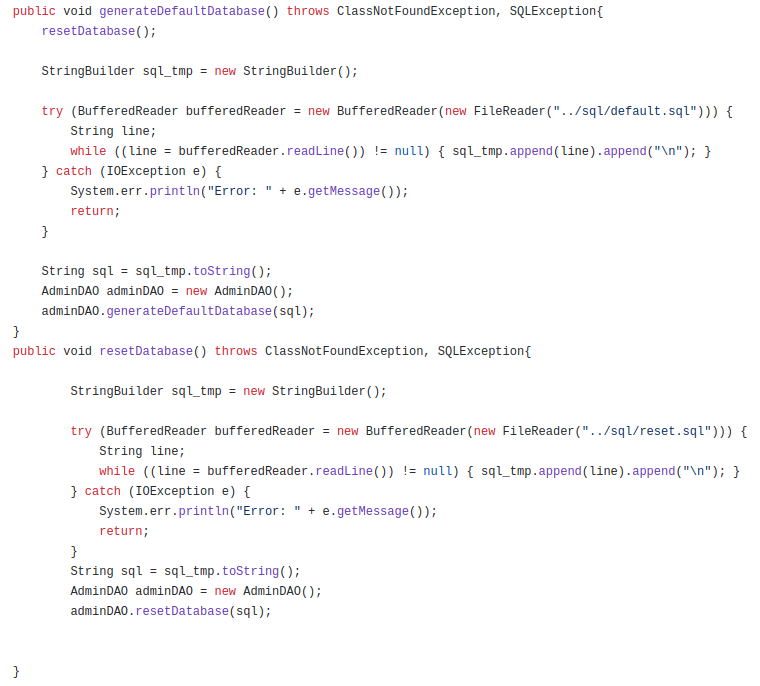
\includegraphics[width=\textwidth]{Images/Snippets/AdminControllerSnippets.png}
                \caption{Snippet: Due delle extra actions}
                \label{fig:admincontrollerSnippets}
            \end{figure}
\subsubsection{UserController}\label{subsubsec:usercontroller}
Controller che gestisce le azioni dell'utente, come il controllo delle proprie prenotazioni e la gestione del proprio profilo. 


\subsubsection{ReserveController}\label{subsubsec:reservecontroller}
Controller che si occupa della creazione, rimozione e modifica delle prenotazione. Chiama \hyperref[subsubsec:resourcescontroller]{\textbf{ResourcesController}} ogni volta che deve fare un accesso a delle risorse. Inoltre è stato qua inserito il metodo di calcolo del costo di una prenotazione, che viene effettuato alla creazione della prenotazione e ogni volta che essa viene modificata. Infine, è stato implementato un metodo che si occupa della gestione della generazione dei \hyperref[subsec:timerecord]{\textbf{TimeRecord}} chiamato \hyperref[fig:fixer]{\textit{TimeRecordFixer()}}, il quale, data in input una data ed un turno, restituisce l'\textit{id} che corrisponde ad esse prendendolo dal \hyperref[subsec:Database]{Database} se già esistente o creandolo sul momento nel caso non sia ancora presente all'interno del sistema.
\begin{figure}[H]
                \centering
                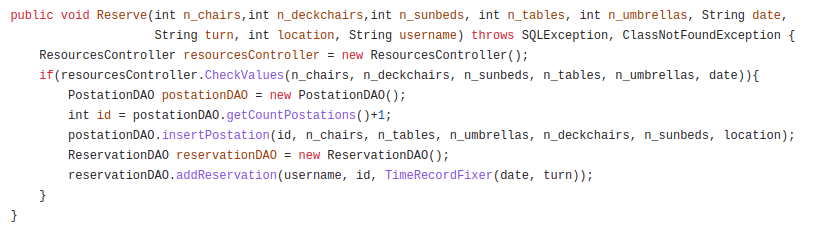
\includegraphics[width=\textwidth]{Images/Snippets/Reserve.png}
                \caption{Snippet: Reserve() method}
                \label{fig:reserve}
            \end{figure}
\begin{figure}[H]
                \centering
                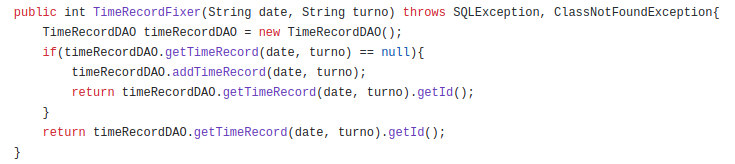
\includegraphics[width=\textwidth]{Images/Snippets/TimeRecordFixer.png}
                \caption{Snippet: TimeRecordFixer() method}
                \label{fig:fixer}
            \end{figure}
\subsubsection{ResourcesController}\label{subsubsec:resourcescontroller}
Controller che si occupa della gestione delle risorse. Il metodo \textit{CheckValues()} viene invocato da \hyperref[subsubsec:reservecontroller]{\textbf{ReserveController}} ogni volta che si richiede di modificare la quantità di risorse all'interno di una prenotazione. Sono inoltre presenti i metodi per la modifica delle risorse presenti nell'impianto balneare e un metodo chiamato \hyperref[fig:getavailableresources]{\textit{getAvailableResources()}} che restituisce il numero di risorse ancora disponibili in una certa data.
\begin{figure}[H]
                \centering
                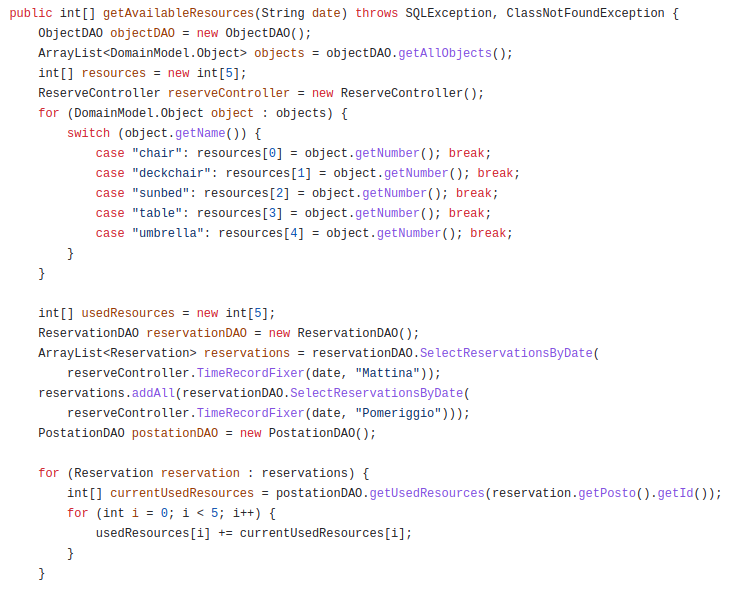
\includegraphics[width=\textwidth]{Images/Snippets/GetAvailableResources.png}
                \caption{Snippet: getAvailableResources method}
                \label{fig:getavailableresources}
            \end{figure}
\subsection{Database}\label{subsec:Database}
Come già accennato nella sezione \hyperref[subsec:ERdiagram]{2.5}, il database è stato progettato in modo da rispettare le specifiche del sistema.
            Sono state create le tabelle \texttt{Users}, \texttt{Location}, \texttt{Object}, \texttt{Reservation}, \texttt{Postation} e \texttt{TimeRecord}
            e sono state definite come indicato nella Figura~\ref{fig:er-diagram-1}.
            I file relativi al database sono contenuti in \texttt{src/sql} e i principali sono \texttt{reset.sql} e \texttt{default.sql}:
            il primo cancella i vecchi dati con il comando \texttt{DROP TABLE IF EXISTS} e ricrea le tabelle secondo la struttura sopra citata,
            mentre il secondo riempe le tabelle con dei dati di default per testare il funzionamento del sistema.
\begin{figure}[H]
                \centering
                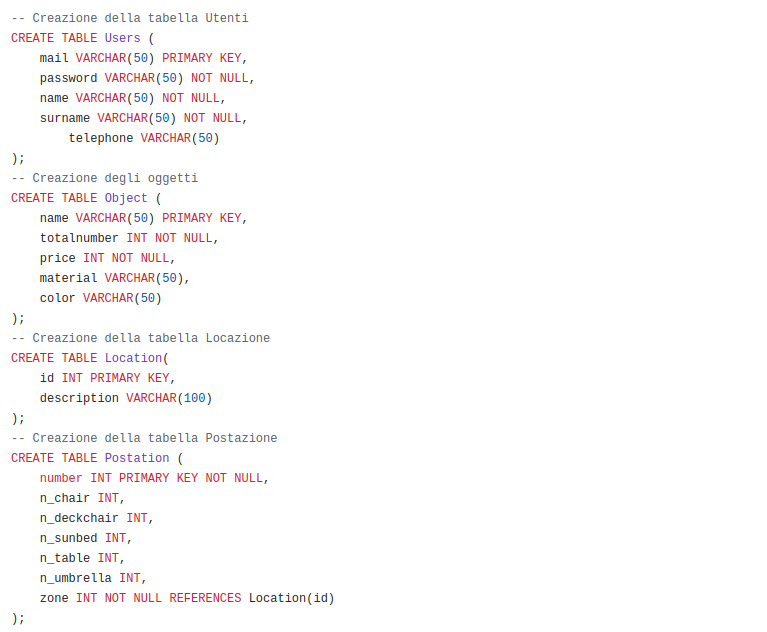
\includegraphics[width=0.9\textwidth]{Images/Snippets/Database.png}
                \captionsetup{labelformat=empty,labelsep=none}
                \caption{Snippet: Database implementation}
                \label{fig:snippetDatabase}
            \end{figure}
\subsection{Interfaccia e CLI}\label{subsec:interfaccia-cli}
Come introdotto nella sezione \hyperref[subsec:struttura-e-pratiche-utilizzate]{1.2}, è stata realizzata un'interfaccia a riga di comando per il sistema, implementata nel file \texttt{Main.java} (il percorso è: \texttt{src/java/Main.java}).
            L'utente può navigare tra le varie pagine e compiere le funzionalità del programma inserendo i vari comandi indicati dal sistema.
            Prendendo per esempio la pagina iniziale \hyperref[fig:navigation-diagram]{\texttt{PoolManager}}, l'utente può scegliere di \hyperref[fig:main]{eseguire l'accesso inserendo il comando \texttt{1}},
            di registrarsi inserendo il comando \texttt{2}, di autenticarsi come admin inserendo il comando \texttt{3} o di uscire dal programma inserendo il comando \texttt{4}.
            Ogni pagina è implementata con un \textit{do-while} e uno \textit{switch-case} per gestire le varie scelte dell'utente, mentre le varie funzionalità
            sono implementate con metodi specifici delle classi del package \hyperref[subsec:BusinessLogic]{\texttt{java.BusinessLogic}}.
            La navigazione tra le pagine avviene tramite chiamate agli stessi metodi della classe \texttt{Main}.
\begin{figure}[H]
                \centering
                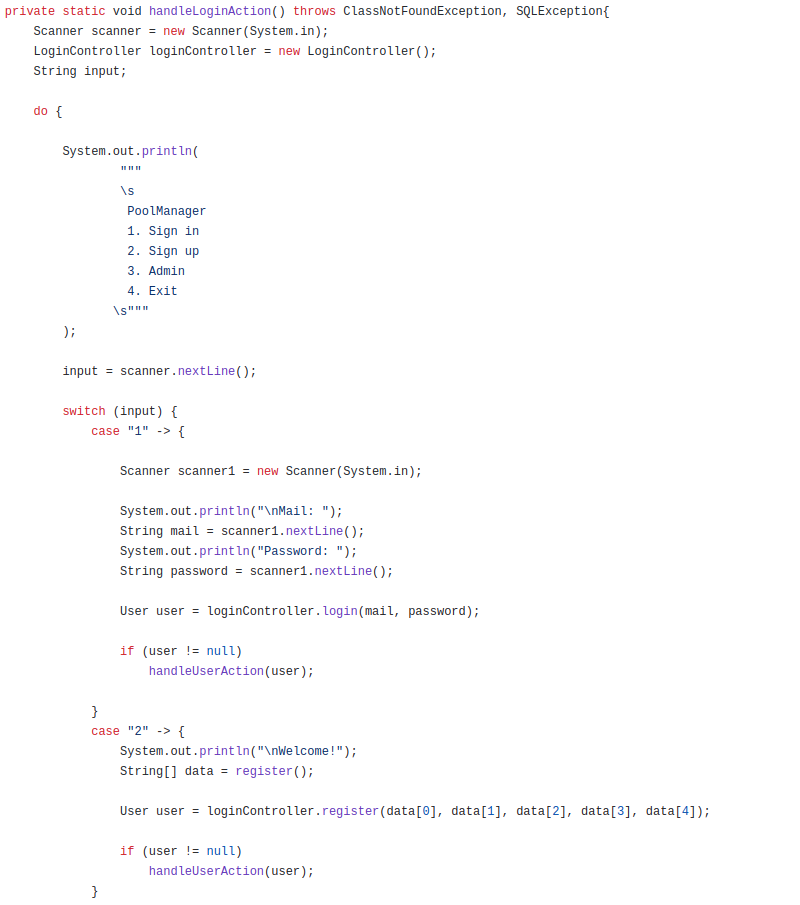
\includegraphics[width=0.9\textwidth]{Images/Snippets/Main.png}
                \captionsetup{labelformat=empty,labelsep=none}
                \caption{Snippet: implementazione della pagina iniziale e della funzionalità di login (Sign in)}
                \label{fig:main}
            \end{figure}
\newpage
\section{Testing}\label{sec:testing}
    Data la struttura del codice, è stato deciso di testare i metodi principali delle classi della \hyperref[subsec:BusinessLogic]{BusinessLogic}, poiché l'implementazione delle classi del \hyperref[subsec:domainmodel]{DomainModel} non ha alcun metodo particolare oltre a \textit{getters} e \textit{setters}. Inoltre i metodi scelti utilizzano diversi metodi di \hyperref[subsec:domainmodel]{DomainModel} e di \hyperref[subsec:ORM]{ORM}, di modo da testare un insieme maggiore di metodi del sistema. Per ogni classe del pacchetto scelto, è stata creata una classe in cui è stato testato almeno un metodo della classe della classe di riferimento. Avendo inoltre implementato tutti i metodi presentati nel \hyperref[subsec:navigation-diagram]{Navigation Diagram}, è stato deciso di formalizzare un minor numero di test rispetto al numero di metodi effettivamente presenti all'interno delle classi.
\subsection{AdminControllerTest}\label{subsec:admincontrollertest}
 Il test scelto per questo controller riguarda il metodo \hyperref[fig:snippetadmindao]{\textit{generateDefaultDatabase()}}, poiché nel farlo è stato possibile testare anche i metodi: \textit{AddUser()}, \textit{getUser()}, \textit{Reserve()} e \textit{getUserReservations()}. Si è quindi controllato che, dopo aver generato il database di default, che si trova al percorso \texttt{src/sql/default.sql}, inserendo un nuovo utente non presente inizialmente non ci fossero prenotazioni a suo nome. Infine si è controllato che, inserita una prenotazione, questa risultasse di fatto all'interno del \hyperref[subsec:Database]{Database}.
\begin{figure}[H]
                \centering
                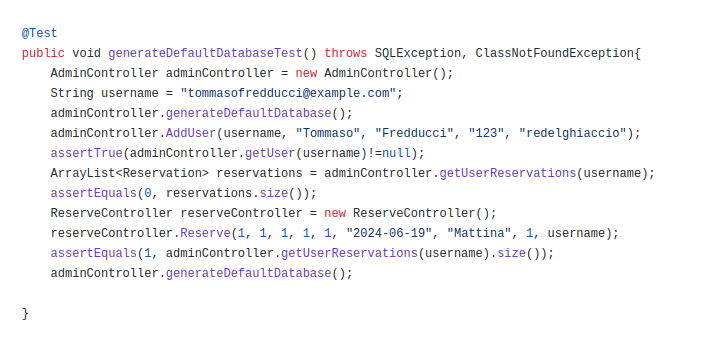
\includegraphics[width=0.9\textwidth]{Images/Snippets/TestAdminController.png}
                \captionsetup{labelformat=empty,labelsep=none}
                \caption{Snippet: test di generateDefaultDatabase()}
                \label{fig:Admincontrollertestsnippets}
            \end{figure}

\subsection{UserControllerTest}\label{subsection:usercontrollertest}
Si è scelto di testare uno dei metodi di aggiornamento del profilo di uno \textbf{User}, prendendo come riferimento il metodo \textit{updatePassword()}, a questa maniera è stato possibile riconfermare il test di \textit{getUser()} e di uno dei \textit{getters} di \hyperref[subsubsec:userDAO]{\textbf{UserDAO}}.
\begin{figure}[H]
                \centering
                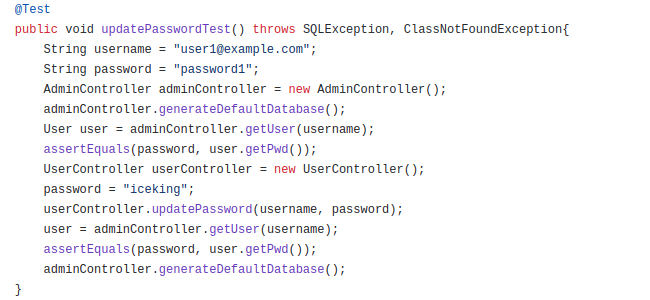
\includegraphics[width=0.9\textwidth]{Images/Snippets/updatePasswordTest.png}
                \captionsetup{labelformat=empty,labelsep=none}
                \caption{Snippet: test di updatePassword()}
                \label{fig:Usercontrollertest}
            \end{figure}
\subsection{ReserveControllerTest}\label{subsection:reservecontrollertest}
Avendo già implicitamente testato il metodo \textit{Reserve()} all'interno del test di \hyperref[fig:Admincontrollertestsnippets]{\textbf{AdminControllerTest}}, è stato qua invece implementato il test di \textit{removeReservation()}. Nello specifico, partendo dalla generazione di un database di default, si salva il numero di prenotazioni totali all'interno di un intero \textit{size}, si procede a rimuovere una prenotazione che conosciamo essere presente all'interno di \texttt{src/sql/default.sql} e si confronta il numero di prenotazioni dopo la rimozione con quello precedente.
\begin{figure}[H]
                \centering
                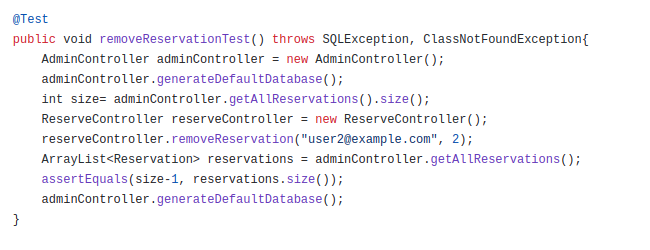
\includegraphics[width=0.9\textwidth]{Images/Snippets/removeReservationTest.png}
                \captionsetup{labelformat=empty,labelsep=none}
                \caption{Snippet: test di removeReservation()}
                \label{fig:ReserveControllerTest}
            \end{figure}
\subsection{ResourcesControllerTest}\label{subsection:resourcescontrollertest}
Per questo controller è stato testato il metodo di controllo dei vincoli sulle risorse \textit{CheckValues()}, andando ad inserire valori che entrano all'interno dei vincoli e valori che fuoriescono dai vincoli.
\begin{figure}[H]
                \centering
                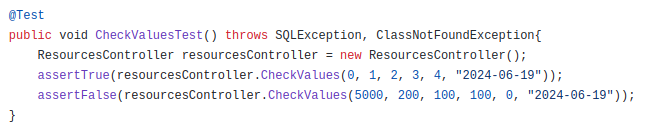
\includegraphics[width=0.9\textwidth]{Images/Snippets/CheckValuesTest.png}
                \captionsetup{labelformat=empty,labelsep=none}
                \caption{Snippet: Test di checkValues()}
                \label{fig:resourcescontrollertest}
            \end{figure}
\subsection{LoginControllerTest}\label{subsection:logincontrollertest}
Per quanto riguarda questo controller, sono stati invece testati i metodi \textit{Login()} e \textit{Register()} andando a controllare che entrambi i metodi risolvessero i propri flussi nella maniera corretta. Nel primo caso, si controlla sia quando si ha un accesso con credenziali corrette, sia quando si cerca di effettuare l'accesso con delle credenziali che non lo sono. Nel caso di \textit{Register()}, invece, si è semplicemente controllato che il metodo restituisse correttamente lo \textbf{User} inserito.
\begin{figure}[H]
                \centering
                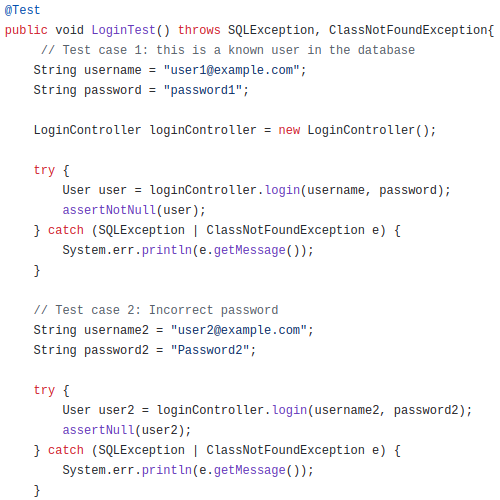
\includegraphics[width=0.9\textwidth]{Images/Snippets/LoginTest.png}
                \captionsetup{labelformat=empty,labelsep=none}
                \caption{Snippet: test di login()}
                \label{fig:logintest}
            \end{figure}
\begin{figure}[H]
                \centering
                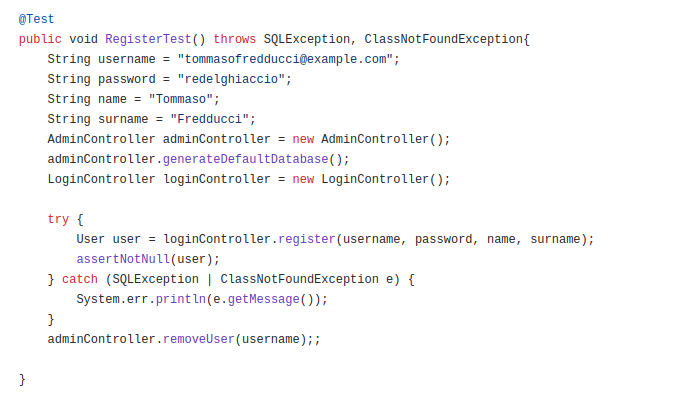
\includegraphics[width=0.9\textwidth]{Images/Snippets/RegisterTest.png}
                \captionsetup{labelformat=empty,labelsep=none}
                \caption{Snippet: test di register()}
                \label{fig:registertest}
            \end{figure}
\end{document}
